\begin{frame}{Le froid}
\only<-4>{\juxt[0.65]{%
\centering%
\vspace{1cm}%
\newcommand{\circulation}{%
\draw (-1.5,1) arc(90:30:2mm);
\draw (-1.515,1.04) -- ++(45:2mm);
\draw (-1.53,1.08) arc(-30:30:2mm);
\draw (-0.08,1.11) arc(-30:30:2mm);
\draw (-0.08,1.1) --++(20:2mm);
\draw (-0.08,1.09) arc(30:-30:2mm);
\draw (-1.39,1.28) arc(0:90:2mm);
\draw (0.42,1.22) arc(0:60:2mm);
\draw (0.45,1.19) --++(40:2mm);
\draw (0.47,1.16) arc(120:60:2mm);
\draw (1.35,0.4) arc(-90:-150:2mm);
\draw (1.375,0.36) --++(-150:2mm);
\draw (1.4,0.32) arc(130:190:2mm);
\draw (1.28,1.35) arc(180:90:2mm);
\draw[opacity=1,line width=0.4pt] (circ) -- ++(1,0) node[pos=1,right,font=\small]{Circulation};
}
\newcommand{\conduction}{%
\draw (-1.1,1.8) -- ++(45:3mm);
\draw (-1.3,1.9) -- ++(80:3mm);
\draw (-1.5,1.8) -- ++(120:3mm);
\draw (-1.7,0) -- ++(180:3mm);
\draw (-1.5,-0.5) -- ++(180:3mm);
\draw (-0.78,-0.2) -- ++(0:3mm);
\draw (-0.5,1.1) -- ++(90:3mm);
\draw (1.28,1.8) -- ++(45:3mm);
\draw (1.15,1.95) -- ++(100:3mm);
\draw (1,1.9) -- ++(120:3mm);
\draw (0.8,0) -- ++(180:3mm);
\draw (0.8,-0.5) -- ++(180:3mm);
\draw (1.45,-1.05) -- ++(45:3mm);
\draw (2,0.7) -- ++(0:3mm);
\draw[opacity=1,line width=0.4pt] (cond) -- ++(1,0) node[pos=1,right]{Conduction};
}
\begin{tikzpicture}[overlay,yshift=3mm]
\node (pic) at (0,0) {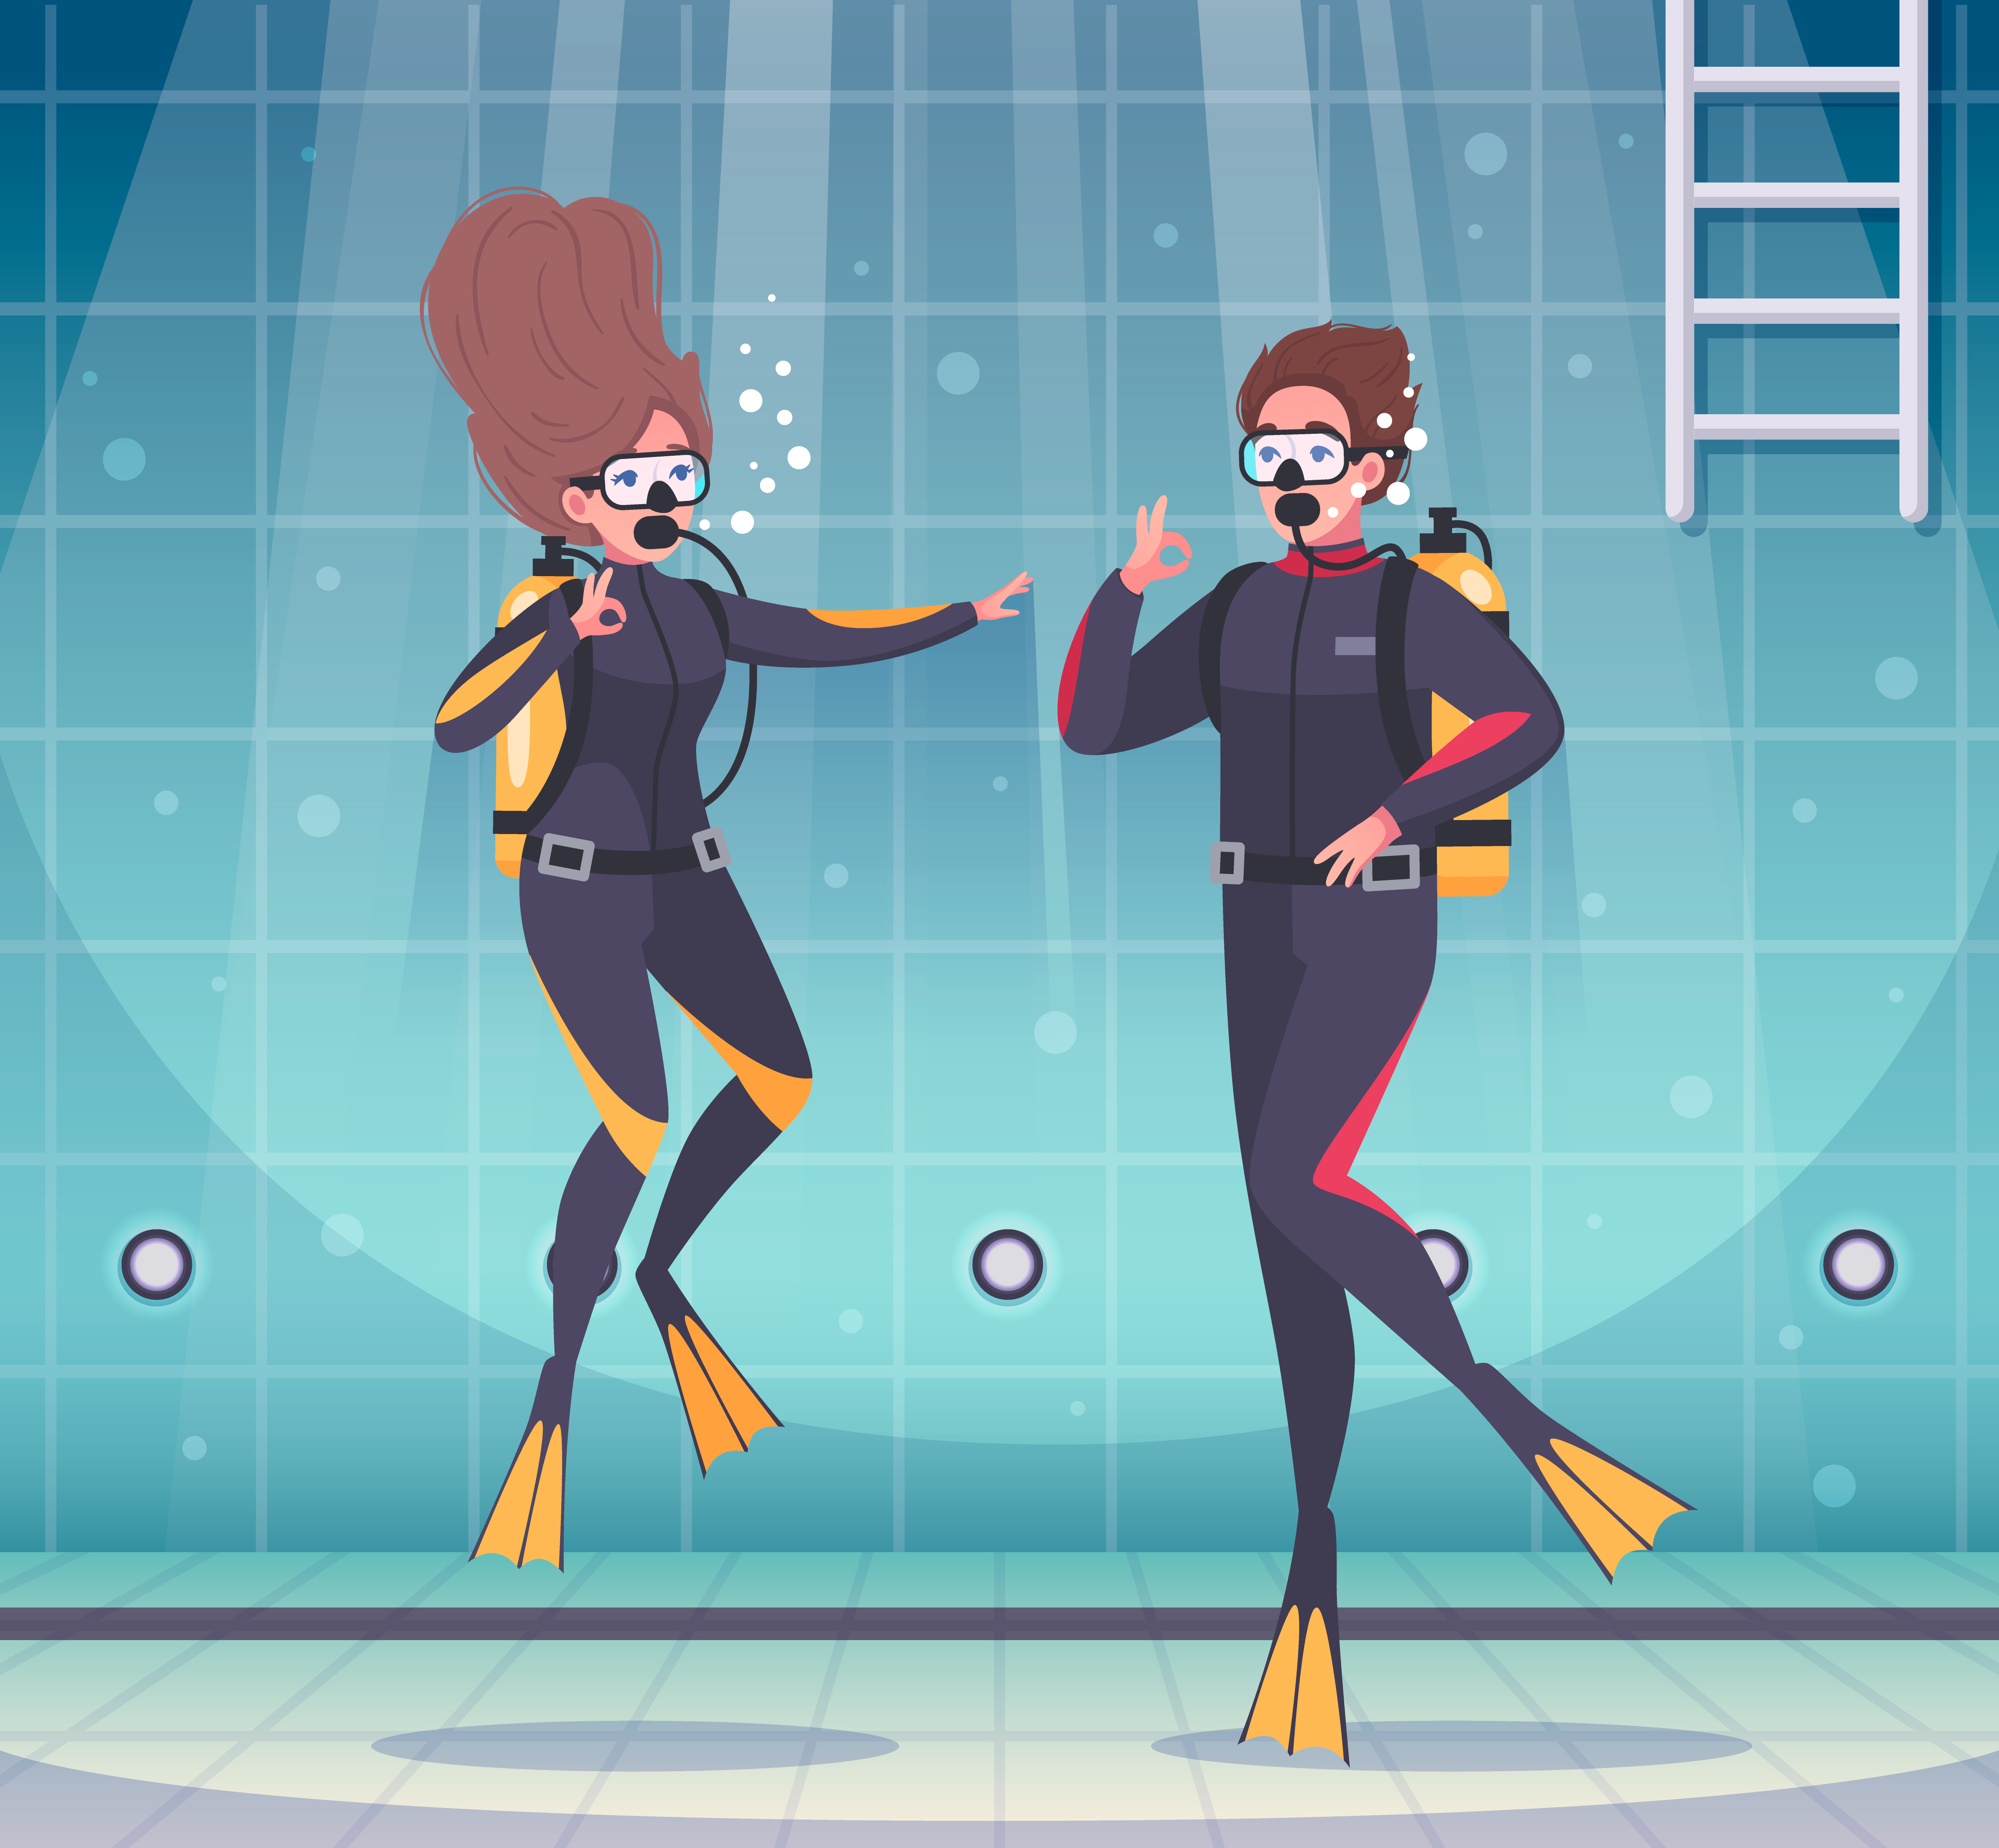
\includegraphics[height=6.5cm]{plongeurs}};
\node[above left=1pt,font=\footnotesize] at (pic.south east) {image: Freepik.com};
\coordinate (circ) at (-3.4,3);
\coordinate (cond) at (-0.2,3);
\coordinate (vent) at (-3.4,2.6);
\temporal<2>{}{%
\begin{scope}[every path/.style={-stealth,thin,blue}]
\circulation
\end{scope}%
}{%
\begin{scope}[every path/.style={-stealth,thin,blue,opacity=0.4}]
\circulation
\end{scope}%
}
\temporal<3>{}{%
\begin{scope}[every path/.style={-stealth,thin,red,decorate,decoration={snake,amplitude=1pt,segment length=3pt, post=lineto, post length=3pt}}]
\conduction
\end{scope}}{%
\begin{scope}[every path/.style={-stealth,thin,red,decorate,decoration={snake,amplitude=1pt,segment length=3pt, post=lineto, post length=3pt},opacity=0.4}]
\conduction
\end{scope}
}
\visible<4>{\begin{scope}[every path/.style={-stealth,thin,yellow,dashed,dash pattern=on 2pt off 1pt}]
\draw (-1.2,1.35) .. controls ++(-0.1,-0.1) .. (-1.3,1);
\draw (-1.2,1.35) .. controls ++(-0.1,-0.1) .. (-1.1,1);
\draw[solid] (-1.2,1.35) .. controls ++(0.3,0.1) .. (-0.8,1.7);
\draw (1.05,1.45) .. controls ++(0.1,-0.1) .. (1.2,1);
\draw (1.05,1.45) .. controls ++(0.1,-0.1) .. (0.85,1);
\draw[solid] (1.05,1.45) .. controls ++(0.2,0) .. (1.35,1.7);
\draw[line width=0.4pt] (vent) -- ++(1,0) node[pos=1,right]{Ventilation};
\end{scope}}
\end{tikzpicture}%
}
{%
\begin{itemize}[<+(1)->]
\item Combinaison bien ajustée. Humide v/s semi-étanche v/s étanche.
\item Épaisseur de la combinaison, souris, cagoule, gants, chaussons néoprène, \dots
\item Pas grand chose à faire\dots
\end{itemize}
}}
\only<5->{%
\juxt[0.4]{\includegraphics[width=\textwidth]{froid}}{%
Refroidissement du corps environ 25 fois plus vite dans l'eau que dans l'air!
\begin{itemize}[<+(5)->]
\item Augmente la consommation,
\item favorise un essouflement.
\end{itemize}
\begin{alertblock}<+(5)>{}
On n'attend pas d'être en hypothermie pour le signaler! Anticiper
le temps de retour et remontée!
\end{alertblock}}}
\end{frame} 
